%#BIBTEX /Library/Tex/texbin/bibtex eccv2016
% last updated in April 2002 by Antje Endemann
% Based on CVPR 07 and LNCS, with modifications by DAF, AZ and elle, 2008 and AA, 2010, and CC, 2011; TT, 2014; AAS, 2016

\documentclass[runningheads]{llncs}
\usepackage{graphicx}
\usepackage{amsmath,amssymb} % define this before the line numbering.
\usepackage{ruler}
\usepackage{color}
% \usepackage{tensor}
\usepackage{algorithm}
\usepackage{algpseudocode}
\usepackage{ulem}
\usepackage{url}
\usepackage[width=122mm,left=12mm,paperwidth=146mm,height=193mm,top=12mm,paperheight=217mm]{geometry}


\algnewcommand\algorithmicforeach{\textbf{for each}}
\algdef{S}[FOR]{ForEach}[1]{\algorithmicforeach\ #1\ \algorithmicdo}

\newcommand{\mysubsubsection}[1]{\vspace{0.2cm} \noindent
\underline{{\bf #1}} \vspace{0.1cm}}
\newcommand{\mysubsubsubsection}[1]{\vspace{0.1cm} \noindent {\bf #1}:}

\newcommand{\pushmeet}[1]{\textcolor{blue}{pushmeet:{#1}}}
\newcommand{\yasu}[1]{\textcolor{magenta}{[yasu: {#1}]}}
\newcommand{\chen}[1]{\textcolor{cyan}{[chen: {#1}]}}
\newcommand{\hang}[1]{\textcolor{green}{[hang: {#1}]}}
%\newcommand{\ikehata}[1]{}
%\newcommand{\yasu}[1]{}
%\newcommand{\hang}[1]{}

\ifx\pdfoptionalwaysusepdfpagebox\relax\else
\pdfoptionalwaysusepdfpagebox5
\fi

\begin{document}
% \renewcommand\thelinenumber{\color[rgb]{0.2,0.5,0.8}\normalfont\sffamily\scriptsize\arabic{linenumber}\color[rgb]{0,0,0}}
% \renewcommand\makeLineNumber {\hss\thelinenumber\ \hspace{6mm} \rlap{\hskip\textwidth\ \hspace{6.5mm}\thelinenumber}}
% \linenumbers
\pagestyle{headings}
\mainmatter
\def\ECCV16SubNumber{***}  % Insert your submission number here

%\title{Parallelizing Hypothesis Fusion for Rapid MAP inference}
\title{Multi-way Particle Swarm Fusion}

\titlerunning{ECCV-16 submission ID \ECCV16SubNumber}

\authorrunning{ECCV-16 submission ID \ECCV16SubNumber}

\author{Anonymous ECCV submission}
\institute{Paper ID \ECCV16SubNumber}


\maketitle

\begin{abstract}
This paper proposes a novel MAP inference framework for Markov Random
Field (MRF) in parallel computing environments.  The inference
framework, dubbed Swarm Fusion, is a natural generalization of the
Fusion Move method. Every thread (in a case of multi-threading
environments) maintains and updates a solution. At each iteration, a
thread can generate arbitrary number of solution proposals and take
arbitrary number of concurrent solutions from the other threads to
perform multi-way fusion in updating its solution. The framework is
general, making popular existing inference techniques such as
alpha-expansion, fusion move, parallel alpha-expansion, and hierarchical
fusion, its special cases. We have evaluated the effectiveness of our
approach against competing methods on three problems of varying
difficulties, in particular, the stereo, the optical flow, and the
layered depthmap estimation problems.
%Our experiments have shown that the Swarm Fusion method outperform
%competing methods, especially for challenging problems with massive
%solution space.
% can effectively exploits the parallel computing resources and become
%effective especially for challenging problems.
%\yasu{must be at least 70 and at most 150 words.}
\keywords{MRF; Fusion Move; Particle Swarm Optimization}
\end{abstract}

\section{Introduction}
Parallel computation has changed the field of computing.  In the 90s,
most processors had single cores. In 2016, most processors have multiple
cores, often 4 or even 8. Cluster computing further expands the
potential of parallel computation, where one can easily launch a
processing job using hundreds or even thousands of computational nodes
in a cloud.
%
In the recent work on the AI program playing the ancient Chinese board
game of {\it Go} (AlphaGo from DeepMind), parallelization plays a key
role in the Monte-Carlo tree search~\cite{nature_alpha_go}.


Parallel computation offers tremendous potential for Computer Vision. As
image sensing technologies have gone through revolutions, we are in
ever growing demands in solving very large problems. One may need to
apply image denoising to 50 Megapixel images from latest digital
SLRs~\cite{canon?}, stitch thousands of images to generate gigapixel
panoramas~\cite{gigapan}, or solve volumetric reconstruction and
segmentation problems over a billion ($=1024^3$)
voxels~\cite{Joint3DSceneReconstructionandclassSegmentation}.
%
%
However, state-of-the-art algorithms are still inherently sequential in
many Computer Vision problems. Take a Fusion Move method
(FM)~\cite{viktor,second_order_stereo,else}, which has been one of the
most effective techniques for the Markov Random Field (MRF) inference,
for example~\cite{fusion_moves}.
%
It sequentially improves solution by fusing the current solution with a
solution proposal. Its successful applications range from optical flow,
stereo, image denoising, image inpainting, to image
segmentation~\cite{fusion_moves_for_markov_random_field_optimization}.


Unleashing the power of parallel computation for effective MRF inference
% Breaking the sequential nature of FM
would then bring fundamental contributions to Computer
Vision. Currently, FM suffers from a few vital limitations due to its
sequential nature. First, standard FM allows only two options per
variable in each fusion, either the current solution or a
proposal~\cite{fusion_moves_for_markov_random_field_optimization}. Second,
only a single proposal generation scheme is used in each fusion
step.~\footnote{Recently, an extension of FM was proposed for layered
depthmap estimation~\cite{chen_2016}, where a solution subspace, instead
of a single solution, is proposed and fused with the current
solution. However, this approach is also limited to the use of one proposal
generation scheme in each fusion.}
%
Our approach, dubbed {\it Swarm Fusion} method (SF), makes a
few key distinctions from existing approaches: 1) Multiple threads (or
computing nodes) simultaneously keep and improve solutions; and 2) Each
fusion in each thread can take arbitrary number of proposals from
arbitrary combination of proposal generation schemes, even concurrent
solutions in the other threads, to be fused with the current solution.
%


We have evaluated the effectiveness of our approach over three problems
in Computer Vision, stereo, optical flow, and layered
depthmap estimation.
%
%Our approach outperforms all the other competing methods, especially for
%challenging problems with a large label space.
Our idea is very simple and the method is easily reproducible with
minimal coding.
% will instantly benefit every Computer Vision researcher or
% engineer, who currently uses fusion move algorithm on multi-core
% environments to solve challenging problems.
% We will share our implementation of the algorithm.


%
% \yasu{Mention that existing fm only does binary solution fusion. We does
% multi-solution fusion. This overlaps withour cvpr16, but is probably ok
% by citing the paepr.}
%
%This paper will propose a novel Parallel Fusion
%Move method, which fuses solution proposals in parallel. Our framework
%can exploit parallelism from the levels of threading to the levels of
%computer nodes.


%The main limitation of FM is its running time, where Computer Vision
%researchers and engineers generally consider FM to be a slow algorithm
%that can solve challenging problems, as hundreds or sometimes thousands
%of proposals need to be fused sequentially.
%


%\yasu{Are there any concrete examples where MRF is used to solve a very
%large problem where parallel fusion is really helpful. Like denoising
%high resolution 24M pixel images. Stitching a high resolution map tiles
%(satellite image tiles) via image stitching.}

%
%This paper will propose a {\it Parallel Fusion Move} (PFM) method that
%introduces the concept of parallel fusion into the computational
%framework.



%
%  \yasu{Hopefully, more interesting things will come up through
% experiments and we have more to say. For example, it would be cool if
% uniform model is better than pure master-slave. Then we can write that
% ours is not just parallel. But keeping multiple solutions somehow
% benefit (GA/GP algorithm's ideas).}


%\yasu{mention GPU somewhere? strange to talk about parallel without
%mentioning GPU and its relation to our approach}



%1. In the introduction, we could mention the recent work on Go (DeepMind's AlphaGo Nature paper) in which parallization plays a key role in the monte carlo search.

%2. Yasu, your explanation of the advantages of Fusion Move (described in
%section 2) is correct. In the sentence on "Second, FM can handle
%problems with very large label spaces.." we could add "and even
%real-valued variables".

%3. I would suggest removing "Genetic algorithms" from the paragraph heading at the end of section 2 or replacing it with "Evolutionary Algorithm".

%4. We should cite two more paper

\section{Related work}


Markov Random Field (MRF) inference has been a very active field in
Computer Vision with extensive literature. We refer the readers to
survey articles for a comprehensive
review~\cite{middlebury_mrf,comparative_study_of_modern_inference}, and
here focus our description on closely related topics.

\mysubsubsection{Parallel Alpha-Expansion}

\noindent Lempitsky et al. introduces parallel computation to an
alpha-expansion technique, where multiple threads simultaneously fuses
mutually exclusive sets of labels. Kumar et
al.~\cite{hierarchical_graph_cuts_kumar_and_koller}, Delong et
al.~\cite{delong}, and Veksler~\cite{olga} proposed an hierarchical
approach, where labels can be simultaneously fused from the bottom to
the top in a tree of labels. 
% 
Instead of taking a hierarchical approach, Batra et
al.~\cite{Dhruv_pushmeet_making_the_right_move} adaptively computed an
effective sequence of labels to explore. This technique can be combined
with parallel alpha-expansion techniques to further obtain speed-up.
%
Strictly speaking, these approaches are not in the family of FM, because
they only consider constant label proposals. Our approach is a
generalization of FM.


\mysubsubsection{Parallel MAP inference}

\noindent
The core MAP inference algorithms themselves can be parallelized.
Strandmark et al. parallelized graph-cuts~\cite{strandmark2010parallel}.
%
Message passing algorithms are friendly to GPU implementation and can
exploit the power of parallel computation.
%
%
While state-of-the-art optimization libraries are often freely available
for non-commercial purposes, most companies have to develop and maintain
in-house implementation of these algorithms.  The core optimization
libraries are often very complex and their modifications require
significant engineering investments for many companies. In contrast, our
idea is extremely simple and easily reproducible by standard engineers.



% \footnote{GPU speeds-up message-passing algorithms via parallel
% computation. However, these algorithms need to store all the messages
% and states and cannot handle problems with a large label
% space~\cite{layered_depthmap}.}


\mysubsubsection{Fusion Move Methods}

\noindent FM was first introduced by Lempitsky et al. in solving an
optical flow problem~\cite{first_fusion_viktor}. FM has been effectively
used to solve challenging problems in Computer Vision such as a stereo
problem with second order smoothness priors~\cite{woodford}, a stereo
problem with parameteric surface fitting and segmentation (i.e., Surface
Stereo)~\cite{surface_stereo}, or multicut
partitioning~\cite{fusionmovesforcorrelationclustering}.
%
FM has two main advantages over the other general inference
techniques~\cite{trw,loopy_belief_propagation}. First, FM allows us to
exploit domain-specific knowledge in customizing proposal generation
schemes. Second, FM can handle problems with very large label spaces
(and even real-values variables), because the core optimization just
solves a binary decision problem.
%
In contrast, methods like message passing algorithms need to maintain
messages and beliefs for the entire label space all the time.
%
Although conceptually straightforward, we are not aware of {\it Parallel
Fusion Move} algorithms that fuses solution proposals, as opposed to
labels, in parallel. This paper seeks to fully unleash the power of
parallel computation in FM via a more general framework.


\mysubsubsection{Evolutionary algorithms and Particle Swarm Optimization}

\noindent
Genetic algorithms (GA)~\cite{ga} and Particle Swarm
Optimization (PSO)~\cite{pso} maintain multiple solutions and improve
them over time.
%
While GA and PSO have limited theoretical justification, they have been
used to produce great empirical results, for example, hand
tracking~\cite{pushmeet_hand_tracking}. At high level, our strategy is
similar in spirit. However, GA or PSO rather arbitrarily copies part of
the solution or makes random movements in each step. Our approach
directly optimizes the objective function to improve solutions.




\section{Multi-way particle swarm fusion} \label{section:algorithm}
Multi-way Particle Swarm Fusion is a natural extension of the Fusion
Move method (FM). We call our method Swarm Fusion (SF) in short. Let us
take multi-threading environment to explain our idea, while the
technique is also applicable to other parallel programming model such as
{\it MapReduce} in cloud computing.
%

Assuming we have $N$ threads $\{T_i | i=1, 2, \cdots, N\}$,
each thread $T_i$ maintains and updates a solution $S_i$ in
parallel.
%Alpha
%Expansion picks one label in each iteration to perform fusion. FM
%generates a solution proposal via a proposal generation scheme.
%invokes one proposal generation scheme and generates a solution proposal
%for fusion.
SF has 1) a {\it proposal generator} for each thread which picks
arbitrary number of proposal generation schemes and generates proposals,
and 2) a {\it solution pool}, from which a thread picks arbitrary number
of intermediate solutions generated by the others.
% threads.
%
% Traditional FM has a set of proposal generation schemes to be
% invoked
%
% There are two places to
% collect solutions or solution proposals for fusion. First, the {\it
% proposal pool} can generate new solution proposals on request.
% %
% Second, the {\it solution pool} stores the solutions that have been
% fused by the threads.
In our base configuration, the solution pool remembers $N$ best
solutions, one from each thread.

SF has two main parameters $\alpha_i$, $\beta_i$ (for each thread
$T_i$), determining its behaviors: In each fusion step, a thread
generates $\alpha_i$ solution proposals using its proposal generator, and collects
% \chen{A proposal pool sounds confusing. We often don't
% really maintain such a pool as many proposals are
% generated dynamically based on current solution. We just
% have certain strategies right there and in each iteration,
% we pick some strategies to generate proposals on the
% fly. This is different with the solution pool which is
% really there.}
$\beta_i$ solutions from the solution pool, based on a user-defined
strategy or at random to be simple. The values of $\alpha_i$ and
$\beta_i$ can vary per iteration for flexibility.
The thread then fuse all these proposals and/or solutions to find a solution
with lower energy state and update the solution pool accordingly.
%
% One can further customize how to pick certain proposal generation
% schemes (as in ~\cite{delong}) or solutions.


Swarm Fusion framework is very flexible and yields various data
processing architectures as shown in Fig.~\ref{fig:model}.
%
\begin{figure}[tb]
 \includegraphics[width=\columnwidth]{figure/model.pdf} \caption{Swarm
   Fusion (SF) architecture and its relationships to existing methods. The
 bottom right example shows the general SF architecture, where
 each thread takes arbitrary number of solution proposals and concurrent
 solutions for fusion. The framework is flexible and
 can realize other data processing architectures depending on the
 parameters (e.g., the left two examples in the bottom row).
 %
 % The left two examples at the
 % bottom row are other Swarm fusion architectures with some restrictions,
 % for which we provide comparative evaluations in
 % Section~\ref{section:results}.
 %
% The left two examples at the bottom are other Swarm fusion
% architectures with some restrictions, to be used for evaluations later.
 %
 It is easy to verify that existing popular MRF inference methods such
 as Alpha Expansion~\cite{alpha_expansion}, Fusion Move~\cite{fusion_moves_for_markov_random_field_optimization},
 Parallel Alpha Expansion~\cite{olga_hierarchical_alpha_expansion}, and Hierarchical
 Fusion~\cite{delong_hierarchical_fusion}, are all special cases of
 SF.}
\label{fig:model}
\end{figure}
%
The bottom right architecture is the most general one, in which
threads conduct multi-way fusion of their current solution, proposals
from their own proposal generators and/or concurrent solutions.
%
For general non-submodular energy, we use TRW-S~\cite{TRW-S, opengm} for inference.
%% And the energy is not submodular
%% in general, for which effective inference techniques such as
%% TRW-S~\cite{TRW-S,opengm} exist.
%
%, and hence we use TRW~\cite{kolmogorov} for the fusion, while any other
%compatible inference techniques can be used~\cite{opengm}.
However, if one knows that a certain fusion step is a binary fusion with
submodular energy, one can use
alpha-expansion~\cite{alpha_expansion}.
%
%If a certain fusion step is a
%binary fusion with non-submodular energy, one can use
%QPBO~\cite{second_order_stereo}.
%
QPBO~\cite{QPBO} can be used to perform binary fusion with non-submodular energy.
Note that the threads appear synchronized in the figure only for
illustration purpose. In practice, all the threads run asynchronously
with a (read-write) lock on the data in the solution pool (See
Algorithm~\ref{algorithm:sf}).
%The asynchronous computing further unleashes the power of parallism.
%The asynchronous processing could be difficult for cloud parallel
%computing.
%
%
%
\begin{algorithm}[t]
 \caption{Swarm Fusion method}
 \label{algorithm:sf}
 \begin{algorithmic}
  %\Procedure{Swarm Fusion method} {}
  \Procedure{} {$\alpha, \beta$}
  \State $\mathcal{S}_{pool} \leftarrow \emptyset$ \ \ \ //Solution pool
  %\State Initialize $\mathcal{P}_{pool}$ // Proposal pool
  \ForEach{thread $T_i$}
  \State Initialize its solution $S_i$
  \EndFor
  \State
  \ForEach{thread $T_i$ in parallel till convergence}
  \State Generate $\alpha_i$ solution proposals $\mathcal{P}$ %\subset \mathcal{P_{\mbox{pool}}}$
  \State Pick $\beta_i$ solutions $\mathcal{S} \subset \mathcal{S_{\mbox{pool}}}$
  \State $S_i \leftarrow \mbox{Fuse}(S_i, \mathcal{P}, \mathcal{S})$
  \State Replaces the solution in $\mathcal{S}_{pool}$ with $S_i$
  %\State [ Generates proposals and update $\mathcal{P}_{pool}$, if necessary ]
  \EndFor
  \EndProcedure
 \end{algorithmic}
\end{algorithm}


\mysubsubsection{Relationships to existing methods}

\noindent It is easy to verify that Alpha-Expansion
(AE)~\cite{alpha_expansion}, Fusion Move
(FM)~\cite{fusion_moves_for_markov_random_field_optimization},
Parallel Alpha Expansion
(PAE)~\cite{fusion_moves_for_markov_random_field_optimization},
and Hierarchical Fusion
(HF)~\cite{delong_hierarchical_fusion,olga_hierarchical_alpha_expansion}
are all special cases of the Swarm Fusion method (SF). AE
can be realized by setting $(\alpha=1, \beta=0)$ and
restricting the proposals to be constant labels with
a single thread. The same goes for FM, this time, without
the restriction on the proposal generation scheme. PAE is
realized by setting $(\alpha=1,\beta=0)$ with multiple
threads, again with a restriction on the proposal generation
scheme (the last sequential fusion in PAE is realized by
$(\alpha=0, \beta=1)$ with a single thread).
%
% The last sequential fusion (at the top of the example in the figure) can
% be modeled by changing to $\alpha=0, \beta=1$ with a single thread.
HF has a slightly different data processing model, without strong ties
between threads and data, but can be realized by setting ($\alpha=2,
\beta=0$) at the bottom level and ($\alpha=0, \beta=2$) at the remaining
levels, while allowing $S_i$ not to be used in the fusion steps of
$T_i$.


% The swarm fusion is highly flexible, and we first introduce our base
% architecture that exploits general strenghts offered by the
% framework. Later, we explain how to further optimize the configuration
% to boost performance for specific problems. In the base architecture,
% all the threads fuse some number of proposals from the proposal pool and
% some number of solutions from the solution pool in each step. In other
% words, all the threads constantly exchange solutions while injecting new
% proposals. This architecture is illustrated in Figure~\ref{fig:model}.


% \begin{figure}[tb]
%   \includegraphics[width=\columnwidth]{figure/model2.pdf}
%  \caption{Base Swarm Fusion architecture.}\label{fig:base}
% \end{figure}

% \mysubsubsection{Relationships to existing methods} Our framework is
% general, and it is easy to verify that existing parallel fusion
% algorithms are just our special cases.
%
% For example, the parallel fusion algorithm by Lempitsky et
% al.~\cite{viktor} always performs binary fusion between the current
% solution and another label, which can be achieved by setting $\alpha_i =
% 1$ and $\beta_i = 0$ for all the threads. The algorithm by
% Veksler~\cite{olga} or Dejong et al.~\cite{dejong} hierarchically fuses
% solutions starting from solution proposals. The algorithm can be
% realized by setting $\alpha_i = 1, \beta_i = 0$ initially, then use
% $\alpha_i = 0, \beta_i=1$  for the rest of the algorithm.

% \noindent
% We now illustrate the power of Swarm Fusion framework for three problems
% in Computer Vision. 


% Suppose $N=4$, $\alpha_1 = 2$, and $\beta_1 = 3$. In this
% configuration, the first thread $T_1$ fuses its current solution $S_1$,
% two new proposal solutions (e.g., by randomly picking two proposal
% generation schemes), and the current solutions $(S_2, S_3, S_4)$ in the
% other three threads. This is a multi-way fusion with a non-submodular
% energy in general, and message passing algorithm such as
% TRW~\cite{kolmogorov} can be used. Sequential QPBO application is
% another.


% Our model is flexible. For example, a parallel fusion move algorithm by
% Lempitsky et al.~\cite{viktor} is a special case of ours, where $\alpha_i$

% , and it is easy to see that 
% Existing parallel fusion techniques are special 

% Our model is flexible and 


\section{Swarm Fusion instantiation}
We compare SF against competing approaches over three problems in
Computer Vision. SF framework has high degrees of freedom and the
challenge is to properly quantity the contributions of various
algorithmic aspects. For this purpose, we have used the three SF
architectures illustrated in Fig.~\ref{fig:model}. For some problems, we
have further limited the capabilities of SF on purpose, to enable
effective and fair comparative evaluations. We now explain the details
of the three problems.

\hang{Better to explain the methology we used, either here or in
  Result part. For example:}

\hang{To evaluate the effectness of different parallel structures, we
  plot the energy minimization process against time. We define the
  energy of the parallel system at a certain time as the minimum
  energy of all threads at that time.}


% We pick three representative problems in Computer Vision to evaluate the
% effectiveness of the Fusion swarm methods against existing methods. We
% control the SF architectures for each problem independently to make
% compa
%
%\yasu{this section is very rough at the moment. requires polishing. but
%algorithms might change as we run experiments.}  We now explain detailed
%implementation of the Swarm Fusion method for three problems in Computer
%Vision (See Fig.~\ref{fig:problem}).  5
\begin{figure}[tb]
 \includegraphics[width=\columnwidth]{figure/problem.pdf} \caption{We
 compare our Swarm Fusion method against competing approaches on a
 depthmap stereo~\cite{middle_bury_stereo}, an optical
 flow~\cite{middlebury_optical_flow}, or a layered depthmap
 estimation~\cite{layered_depthmap} problem. In the layered depthmap
 problem, the input is an RGBD image, and the output is multiple layeres
 of depthmaps. Each layer is a piecewise smooth parametric surface
 model.}\label{fig:problem}
\end{figure}



\subsection{Swarm Fusion stereo}
We start with a simple depthmap stereo problem with standard unary and
pairwise terms. We employ submodular pairwise terms to make this stereo
represent relatively ``easy'' MRF inference problems.
%
Unary terms are computed as the average robust photoconsistancy
score~\cite{woodford} between the reference image and the others inside a $7\times 7$
pixels window.
\begin{equation}
  \text{\hang{equation to fill in}}
\end{equation}
Pairwise terms are simple truncated absolute label
difference with maximum label difference $\sigma_s=4$. The total energy is
defined by the sum of the two, while scaling the pairwise term by a
factor of $0.005$. For simplicity we don't enforce visibility constraint.

%
We performed our experiments on Book sequence from Middlebury stereo datasets.~\cite{middlebury_stereo}.

\mysubsubsection{Competing methods}

\noindent The sophistication of photometric consistency
function~\cite{mvs_furukawa_survey} makes unary terms dominant in most
stereo problems.  Our experiments have also supported this, where the
fusion method (i.e., the use of proposal generation) rather makes it
slow due to the overhead.\hang{Don't quite understand this
  sentence. Does the ``dominant'' means running time or energy? In my
  experiments, unary terms are pre-computed and are not counted into
  the running time} Therefore, we have chosen Parallel Alpha
Expansion~\cite{delong} and Hierarchical Fusion~\cite{delong,olga}
with graph-cuts optimization as the competing methods.

Since the optimization in the above stereo problem is fairly easy, we
compare our method with standard sequential alpha expansion, parallel
alpha expansion \cite{first_fusion_viktor} and hierarchy fusion
\cite{olga}. In all experiment, we use $\alpha$-expansion to fuse
single label proposals, and QPBO to fuse multi-label proposals. 


\mysubsubsection{Swarm Fusion architectures}

\noindent The three swarm architectures in Fig.~\ref{fig:model} have
been evaluated: SF-SS (SF without solution sharing), SF-MF (SF without
multi-way fusion), and the standard SF.
%
SF-SS implies $\beta=0$, where $\alpha$ is the free parameter and set to
2. SF-MF implies $\alpha+\beta=1$, where each thread iterates the step
of ($\alpha=1, \beta=0$) or ($\alpha=0, \beta=1$) so that it can take a
solution proposal in one step and a neighboring solution in the
next. For standard SF, we have used ($\alpha=1, \beta=1$).


after 4 iterations (alpha, beta),

%
%
%
%
To make the comparison simple, we restrict our proposal
generation to be constant-label proposals. Graph-cuts is used in fusing
a constant-label proposal as the energy is submodular. QPBO is used in
fusing a different solution from another thread as the energy is
non-submodular.
%
% Due to the lack of multi-way fusion, the swarm fusion architecture for
% the stereo problem is represented by the middle example at the bottom of
% Fig.~\ref{fig:model}.

\subsection{Swarm Fusion optical flow}

Fusion Move was first introduced by Lempitsky et al.~\cite{fusion_flow} to
solve the optical flow problem.
% Optical flow was the problem, in which the Fusion Move method was first
%introduced by Lempitsky et al.~\cite{viktor}.
We copy their problem setting and use images from the Middlebury optical
flow benchmark~\cite{middlebury_optical_flow}. We share similar proposal
generation schemes with Lempitsky et al~\cite{fusion_flow}
%instead of the HS algorithm, we
 with some modifications.~\footnote{First, we use more recent
   Farneback algorithm and change the level of pyramids from 1 to 5,
   then use either 3, 5 or 7 for parameter ``polyN''. Besides the
   clustering idea, we add three simple proposal generation schemes
   based on the current solution as suggested in
   \cite{fusion_flow}. In \textit{shift proposal}, the flow field in
   the current solution is shifted in either x or y directions for
   either 1, 2 or 3 pixels. In \textit{stagger proposal}, the flow
   field is shifted by a vector randomly drawn from a Gaussian
   distribution. In \textit{perturb proposal}, each flow value in the
   field is independently shifted by a vector randomly drawn from a
   Gaussian distribution. We choose schemes randomly when generating
   proposals.}

\mysubsubsection{Competing methods}

\noindent Fusion Move method in Lempitsky's paper is the first natural
contender. While they did not consider parallel implementation, it is
straightforward to combine the idea of Parallel Alpha Expansion and
Fusion Move. Therefore, the second competing method is ``Parallel Fusion
Move''(PFM), which is equivalent to Parallel Alpha Expansion with constant
label solutions replaced by solution proposals.
%each thread repeats generating
%a solution proposal and fusing it to the current solution. Solutions
%from all the results are sequentially fused to obtain the final solution
%as in the Parallel Alpha-Expansion method.
%
One problem of PFM is that infinite number of solution proposals can be
generated in their algorithm, and we do not know when to stop and
perform the final sequential fusion (See Parallel Alpha Expansion
architecture in Fig.~\ref{fig:model}). In our experiments, we manually
picked time limits to initiate the final fusion to make the comparisons
fair.
%In Fig.~\ref{fig:model}, this computational framework corresponds to
%``parallel alpha-expansion'' with the label solutions replaced by
%solution proposals.
%
The last contender is the mix of the Hierarchical Fusion and the Fusion
Move methods, dubbed ``Hierarchical Fusion Move''(HFM), where they
start from solution proposals as opposed to constant labels. One problem
of HFM is that we need to generate all the proposals first to build the
fusion tree. This undermines the power of fusion move that can
adaptively generate proposals based on the current solution. In our
experiments, we have manually generate 250 proposals at the
beginning.
%We first generate 25 proposals using LK and Farneback algorithms which
%are independent and generate other proposals based on these initial
%proposals).
The fusions are binary in these methods and we have used QPBO.

\mysubsubsection{Swarm Fusion architectures}

\noindent
%The three swarm fusion models (at the bottom of Fig.~\ref{fig:model})
%are used to evaluate the effectiveness of our method.
The three swarm architectures in Fig.~\ref{fig:model} (SF-MF, SF-SS, SF)
have been evaluated against the competing methods. For SF-MF, each
thread repeats generating solution proposals ($\alpha=1, \beta=0$) for
four iterations and fuses with one solution from others ($\alpha=0,
\beta=1$) in one iteration. This pattern is repeated. For SF-SS, each
thread generates three solution proposals for fusion in each iteration
($\alpha=3$, $\beta=0$). For SF, we repeat four iterations of
($\alpha=3, \beta=0$) and  one iteration of ($\alpha=0, \beta=3$).
%%
%Note that we have used the same set of proposal generation schemes as
%the competing methods.
We have used TRW-S for multi-way fusion and QPBO for binary fusion.
% , while our fusions are multi-way, for which we have used TRW-S.
%
% The full swarm fusion model (at the bottom right in
% Fig.~\ref{fig:model}) will be used to evaluate the effectiveness of our
% method. We will also try the other two Swarm fusion variants in
% Fig.~\ref{fig:model} with restrictions.
%
% 2 k-way 1 solution sharing. \chen{?}

\subsection{Swarm Fusion layered depthmap estimation}

Our last problem is layered depthmap estimation, recently proposed
in~\cite{layered_depthmap} (see the anonymous paper in the
supplementary material).  The problem seeks to infer layered depthmap
representation from an RGBD image, where each layer is a piecewise
smooth segmented depthmap. This is essentially a multi-layer extension
of Surface Stereo algorithm~\cite{surface_stereo}.
%
Layered depthmap estimation is one of the most difficult kinds in MRF
inference due to its massive solution space \chen{and complex energy function?}. The number of labels per
pixel is exponential in the number of layers, and is an order of 100,000
\yasu{is this number correc?} \chen{The number is correct but ``an order of'' sounds strange to me. Maybe say: usually between 100,000 and 10,000,000.}. We copy their problem
formulation and the proposal generation schemes.~\footnote{Authors have
proposed a novel fusion scheme, where a solution subspace instead of a
single solution is generated by a proposal generation scheme. Since a
solution subspace is equivalent to multiple solution proposals \chen{It is a good explanation for this paper's purpose, but from the perspective of our previous work, I am reluctant to say a subspace equals to multiple solution proposals. When we design proposals, we find the subspace directly and there's no concept of solution proposals (we later simplify our subspace proposals to binary labels just for the comparison reason). It is essentially the same, but a subspace proposal is conceptually more general than concatenated solution proposals.}, their
algorithm can be easily integrated into our swarm fusion framework.
However, competing fusion methods (e.g., Parallel Fusion Move or
Hierarchical Fusion) cannot handle a solution subspace proposal, making
it impossible to conduct fair comparative evaluations. We choose to use
a simple solution proposal for experiments in this paper.}
%Lastly, we will evaluate Swarm fusion on a very challenging layered
%depthmap estimation problem~\cite{layered_depthmap}, which has been
%recently proposed (see the anonymized pdf in the supplementary
%material).

\mysubsubsection{Competing methods}

\noindent Solution proposals depend heavily on the current solution,
eliminating the possibility of using Hierarchical Fusion, which needs to
enumerate all the proposals to start. Therefore, viable competing
methods are Fusion Move and Parallel Fusion Move.
%
%We will also evaluate the standard Fusion Move method.
%
The fusions are binary, for which we use QPBO.

%The number of labels is extremely large (an order of 10,000 \yasu{what
%were the number of labels in our cvpr16?}), which eliminates the
%possibility of using hierarchical fusion. Therefore, we will evaluate
%fusion move and parallel fusion move algorithm as in the case of optical
%flow problem, where one solution proposal repeats being fused via QPBO.


\mysubsubsection{Swarm fusion architectures}

\noindent The three swarm architectures with the same configurations as
in the optical flow problems have been evaluated. \chen{same with optical flow, but slightly
  different with stereo (1 sharing in 3 iterations instead of 5 iterations).}
%in Fig.~\ref{fig:model} are evaluated.
%The architecture parameters are exactly the same as in the optical flow problem:
%$\alpha=2$ ($\beta=0$) in SFWSS, the iteration of
%($\alpha=1, \beta=0$) and ($\alpha=0, \beta=1$) in SFWMF, and
%($\alpha=1, \beta=1$) for the standard SF.
%
%The fusions are multi-way, for which we use TRW-S.


\section{Experimental results}
\label{section:results}
We have implemented the algorithms with multithreading supporting from
C++ 11 and conducted the experiments on Linux PCs with Intel Core i7
4790 processor with 4 cores, enabling 8 threads with the hyper
threading technology. We have used the Graph-cuts optimization code
written by Veksler, using the libraries provided by Boykov and
Kolmogorov~\cite{middlebury_mrf,2,3,4_below}.
% [2] Fast Approximate Energy Minimization via Graph Cuts.
%         Y. Boykov, O. Veksler, and R. Zabih.
%         In IEEE Transactions on Pattern Analysis and Machine Intelligence
%         (PAMI), vol. 23, no. 11, pages 1222-1239, November 2001.  
%
%     [3] What Energy Functions can be Minimized via Graph Cuts?
%         V. Kolmogorov and R. Zabih. 
%         In IEEE Transactions on Pattern Analysis and Machine Intelligence
%         (PAMI), vol. 26, no. 2, pages 147-159, February 2004. 
%         An earlier version appeared in European Conference on Computer
%         Vision (ECCV), May 2002.
%
%     [4] An Experimental Comparison of Min-Cut/Max-Flow Algorithms for
%         Energy Minimization in Vision. 
%         Y. Boykov and Vladimir Kolmogorov.
%         In IEEE Transactions on Pattern Analysis and Machine Intelligence
%         (PAMI), vol. 26, no. 9, pages 1124-1137, September 2004. 
We have used the QPBO and TRW-S implementations by
Kolmogorov~\cite{}.

\mysubsubsection{Stereo}

\noindent We have chosen 7 images with the resolution of $695\times555$
from the Book sequence of Middlebury stereo dataset for our
experiment~\cite{middlebury_stereo}. The number of disparity labels is
set to 256.
%
Since the order of labels is important for the expansion techniques,
we have used the same random order for all algorithms to avoid any
bias.
%
% In PAE, SF-MF, SF-SS and SF algorithms, the proposal generator in each
% thread can only generate constant-label proposals within a evenly split
% subset of all labels.



Fig.~\ref{fig:stereo_global} compares the converegence rate of the
competing methods. Note that we define the energy of a multi-threading
system to be the energy of the best solution found so far.
%
\begin{figure}[tb]
  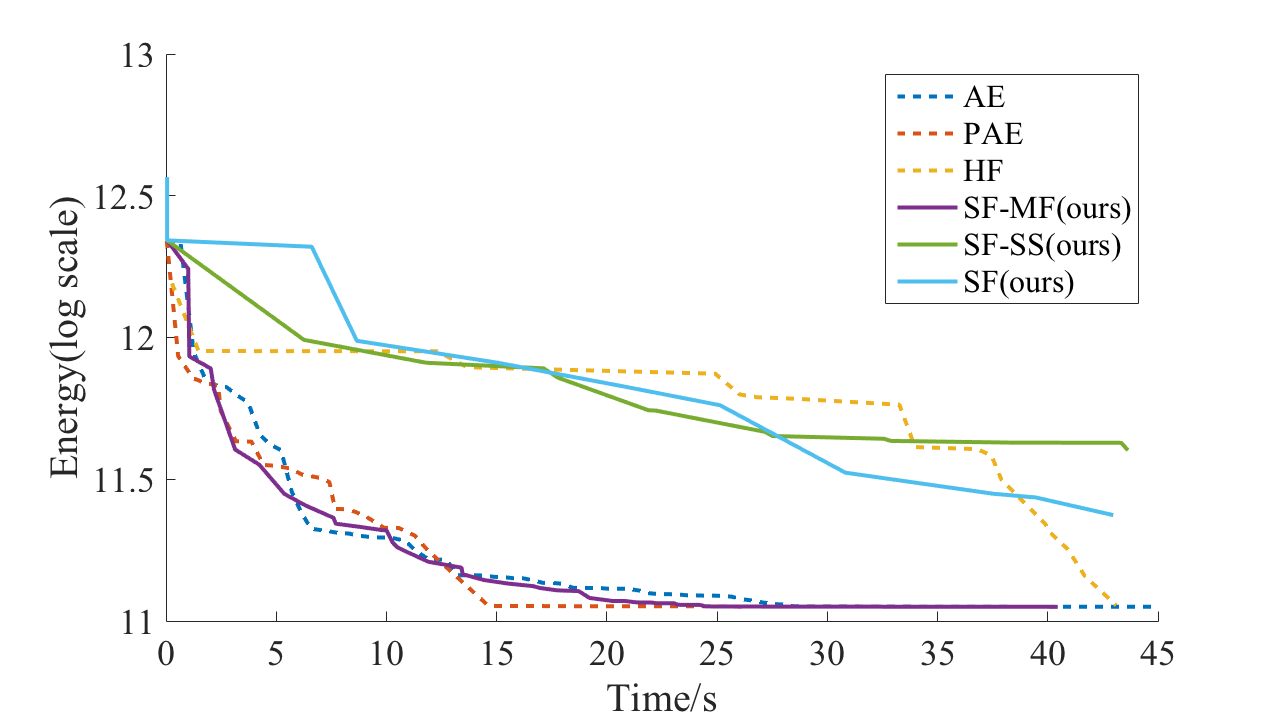
\includegraphics[width=\columnwidth]{figure/stereo_global.png}
 \caption{Energy plots for the stereo problem. The energy is in the log
 scale. For a multi-threading algorithm, the energy at a given moment is
 defined to be the best solution so far.} \label{fig:stereo_global}
\end{figure}
%
One unusual outcome is that Sequential Alpha Expansion and Parallel
Alpha Expansion (PAE) have the same convergence speed, indicating that
the stereo problem is a very easy one.
%This is well known in a community and this fact was rather expected.
Our approaches with multi-way fusion (SF-SS or SF) are the slowest kind,
because the TRW-S for multi-way fusion is slower than multiple Alpha
Expansion steps, and this stereo problem is too easy to gain benefits
through mulit-way fusion.
%
%Another interesting observation is that the Hierarchical Fusion can
%achieve good energy only when they merge solutions at the top of the
%tree.
%
%  both PAE and SF-MF converge faster
% than sequential method. However, since fusing solutions with multiple
% labels by QPBO is slower than a single $\alpha$-expansion, PAE method
%
% Finally, the line of hierarchy fusion only makes
% jump when fusing on root node of the tree. This is because any fusion
% step on non-root nodes only have partial label information.
%We recoreded both single thread energy and system energy against
%time.
%
Fig. \ref{fig:stereo_threads} shows the energy plot per thread
for SF-MF (ours) and PAE. The graph for PAE again confirms that the
stereo is an easy problem, because all the threads are quickly
converging to a solution before the final sequential fusion.
%shows the per-thread energy
%minimization process in SF-MF and PAE. The per-thread energy in SF-MF
%architecture decreases more uniformly than that of PAE. In the
%scenario where we need to query the best solution so far before the
%whole optimization converges, SF-MF architecture is a better choice.
\begin{figure}[tb]
  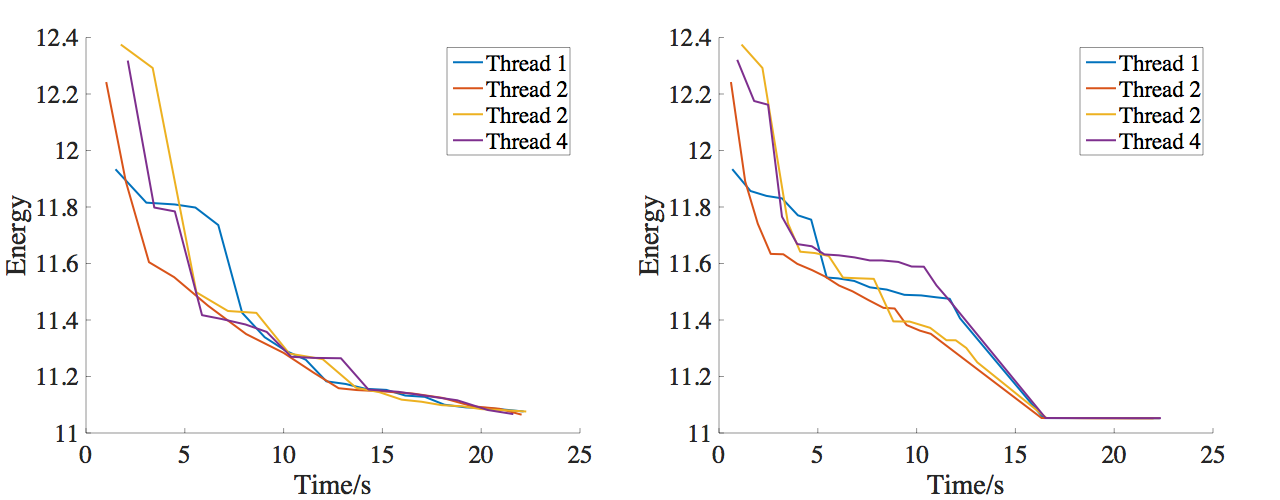
\includegraphics[width=\columnwidth]{figure/stereo_threads.png}
  \caption{Energy plots per thread for the stereo proble for SF-MF (left) and
 Parallel Alpha Expansion (right).
} \label{fig:stereo_threads}
\end{figure}

For an easy optimization problem such as stereo with strong unary terms
and submodular pairwise terms, our full architecture with solution
sharing and multiway fusion actually makes convergence slower due to the
overhead of fusion and multi-threading.




% over-sophisticated fusion algorihtm and multi-threading
% overhead. However, we can easily configure the architecture to make it
% better fit the problem, e.g. turn off multiway fusion and/or solution
% sharing.





% We define the energy of
% a parallel optimization system at a certain time as the minimum energy
% of all threads at that time.


The figure illustrates the convergence rate of three competing methods
(alpha expansion, parallel alpha expansion, hierarchical fusion) against
our swarm fusion method.

%\hang{figure file missing}
\begin{figure}[tb]
  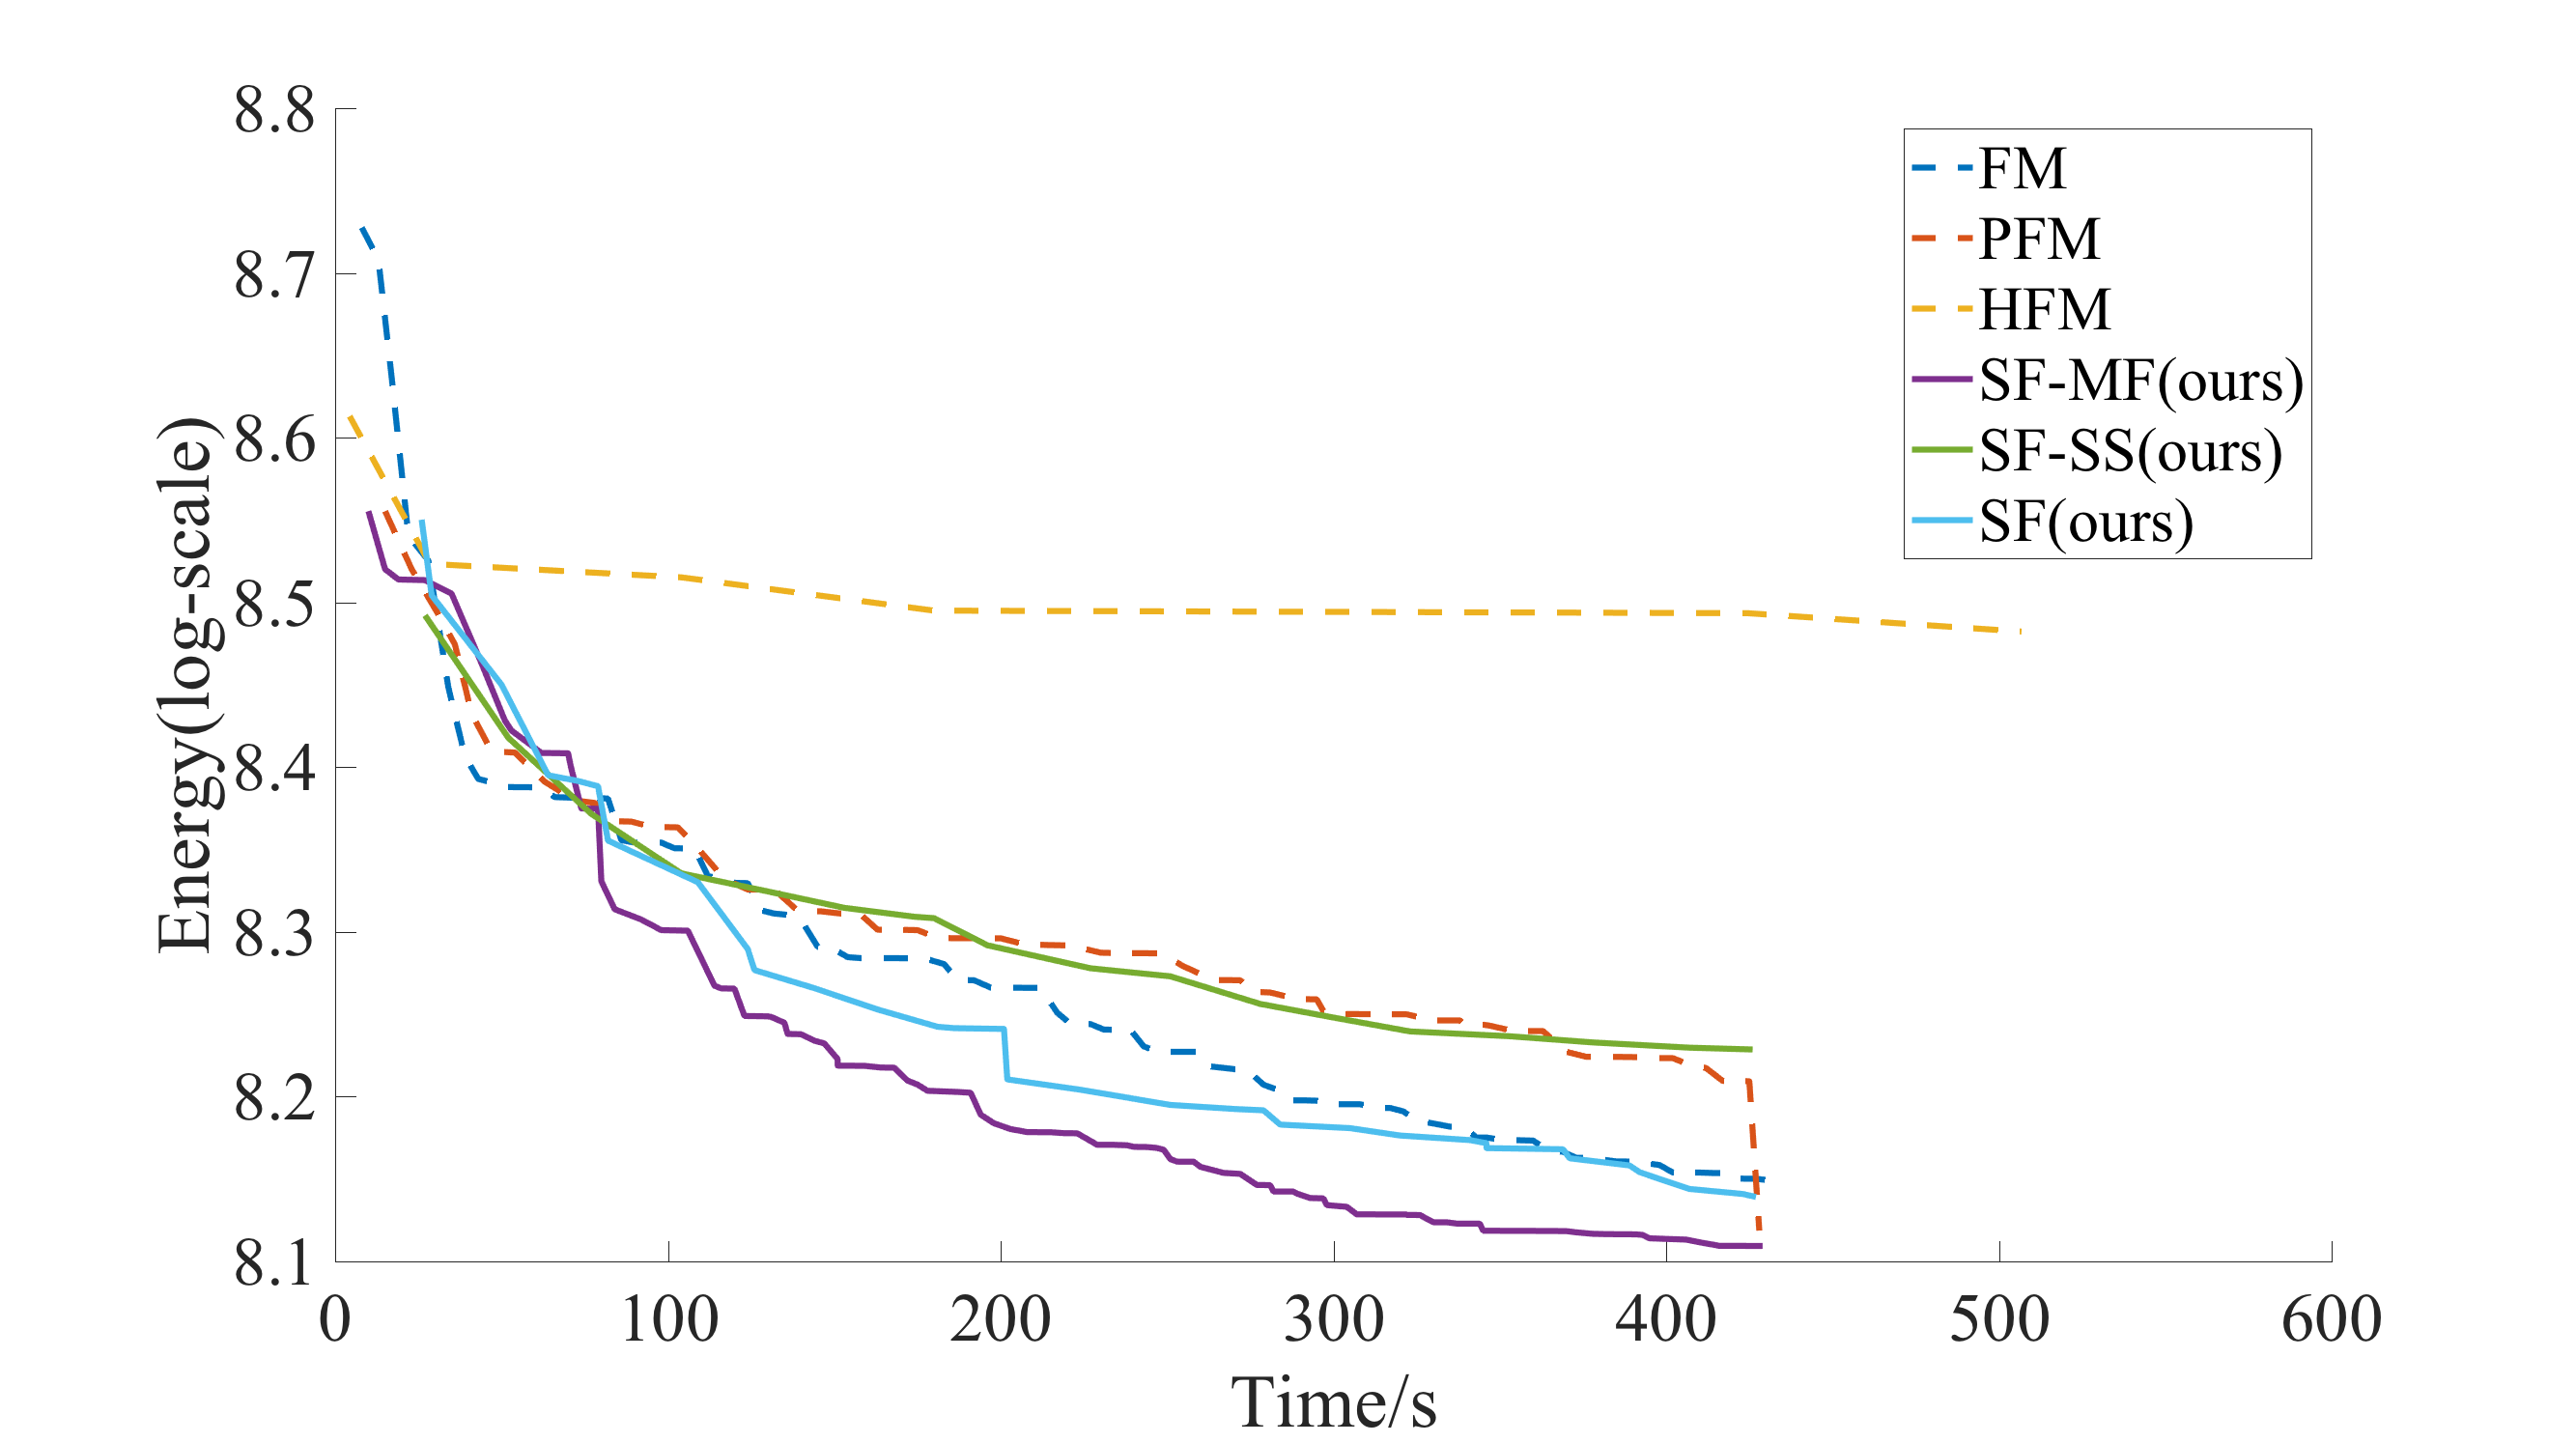
\includegraphics[width=\columnwidth]{figure/optical_flow_convergence.png}
  \caption{}\label{fig:optical_flow_convergence}
\end{figure}
\begin{figure}[tb]
 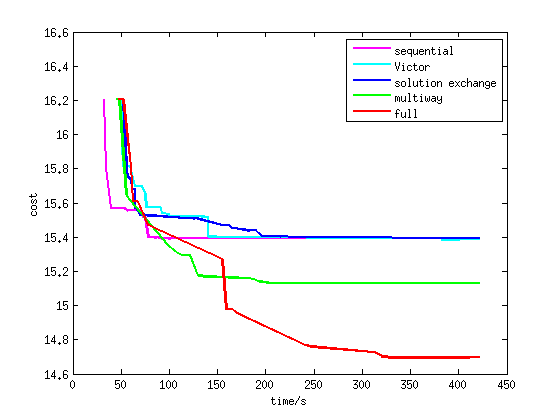
\includegraphics[width=\columnwidth]{figure/layered_depthmap_convergence.png}
 \caption{}\label{fig:layered_depthmap_convergence}
\end{figure}
\begin{figure}[tb]
  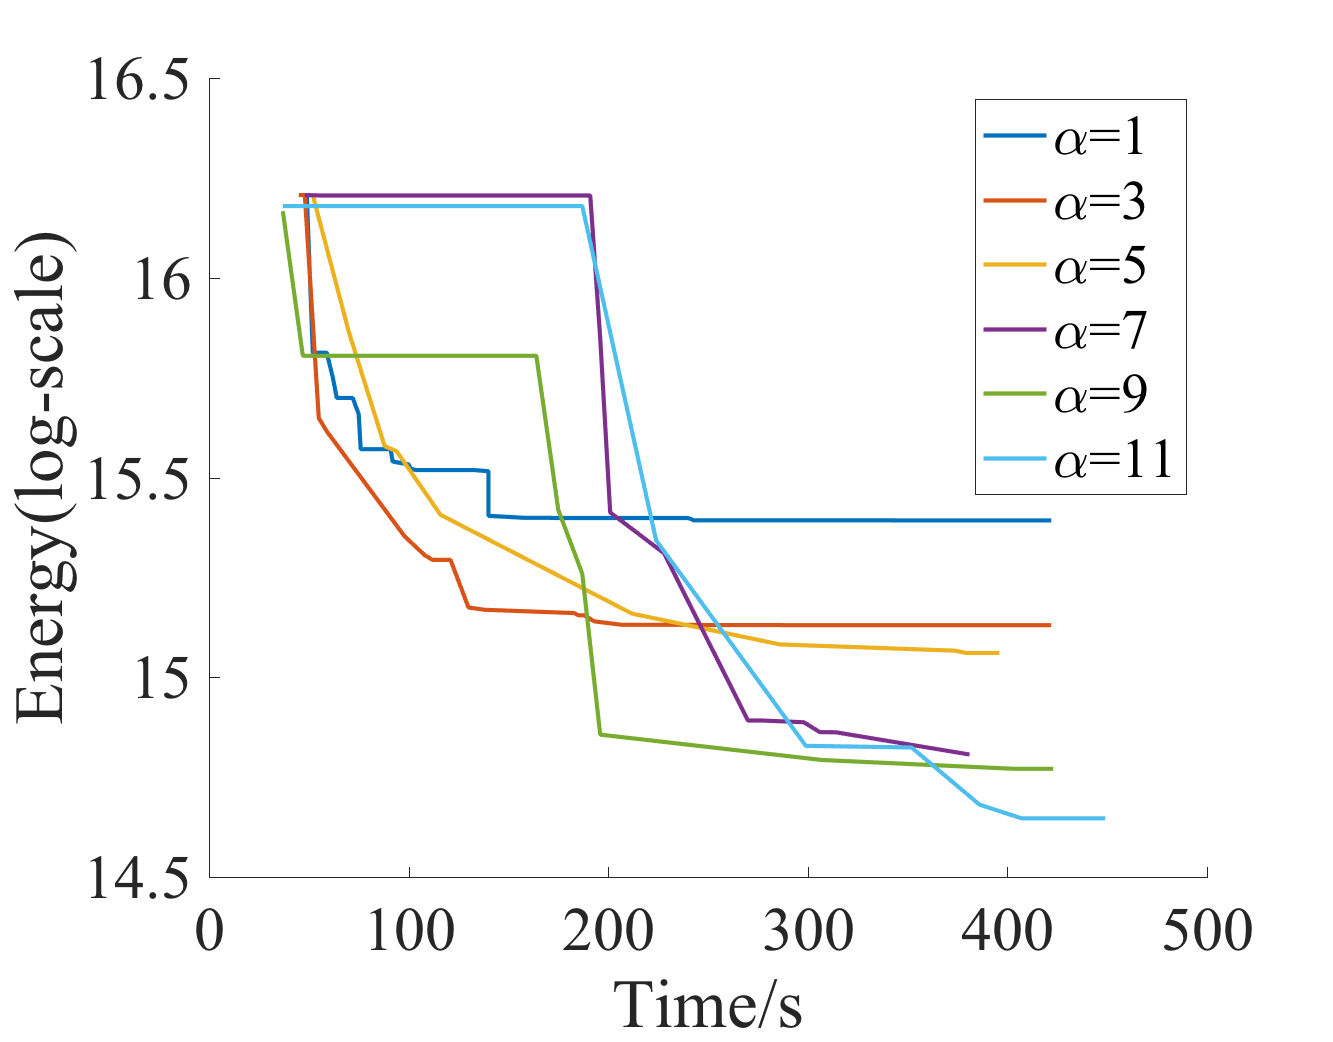
\includegraphics[width=\columnwidth]{figure/layered_depthmap_by_alpha.png}
  \caption{}\label{fig:layered_depthmap_by_alpha}
\end{figure}
\begin{figure}[tb]
  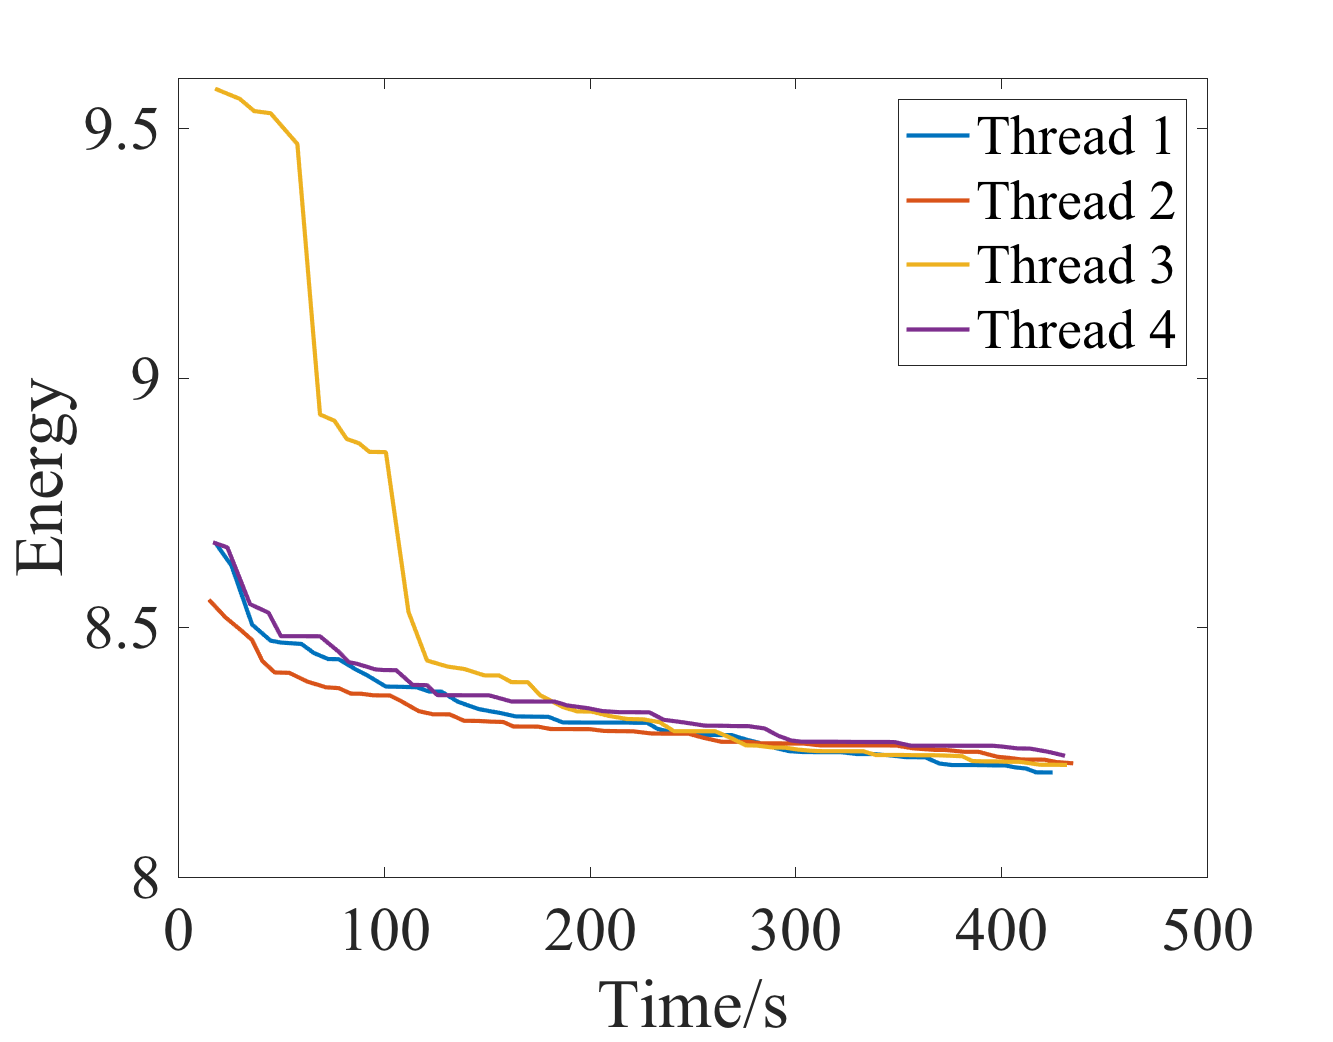
\includegraphics[width=\columnwidth * 0.5]{figure/optical_flow_PFM_threads.png}
  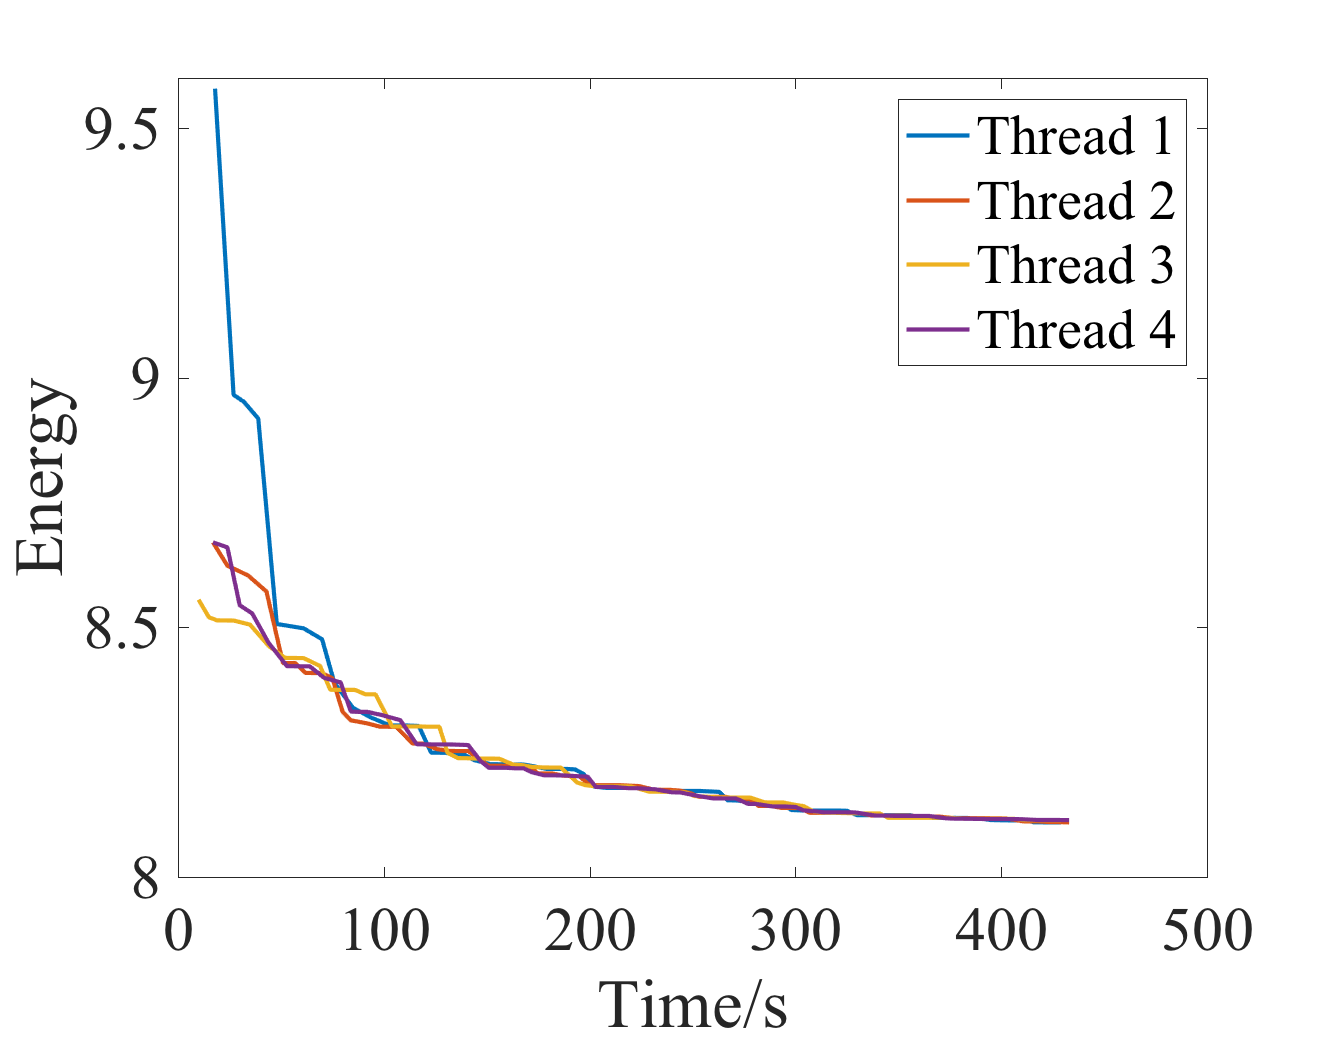
\includegraphics[width=\columnwidth * 0.5]{figure/optical_flow_SF_MF_threads.png}
  \caption{}\label{fig:optical_flow_by_threads}
\end{figure}
\begin{figure}[tb]
  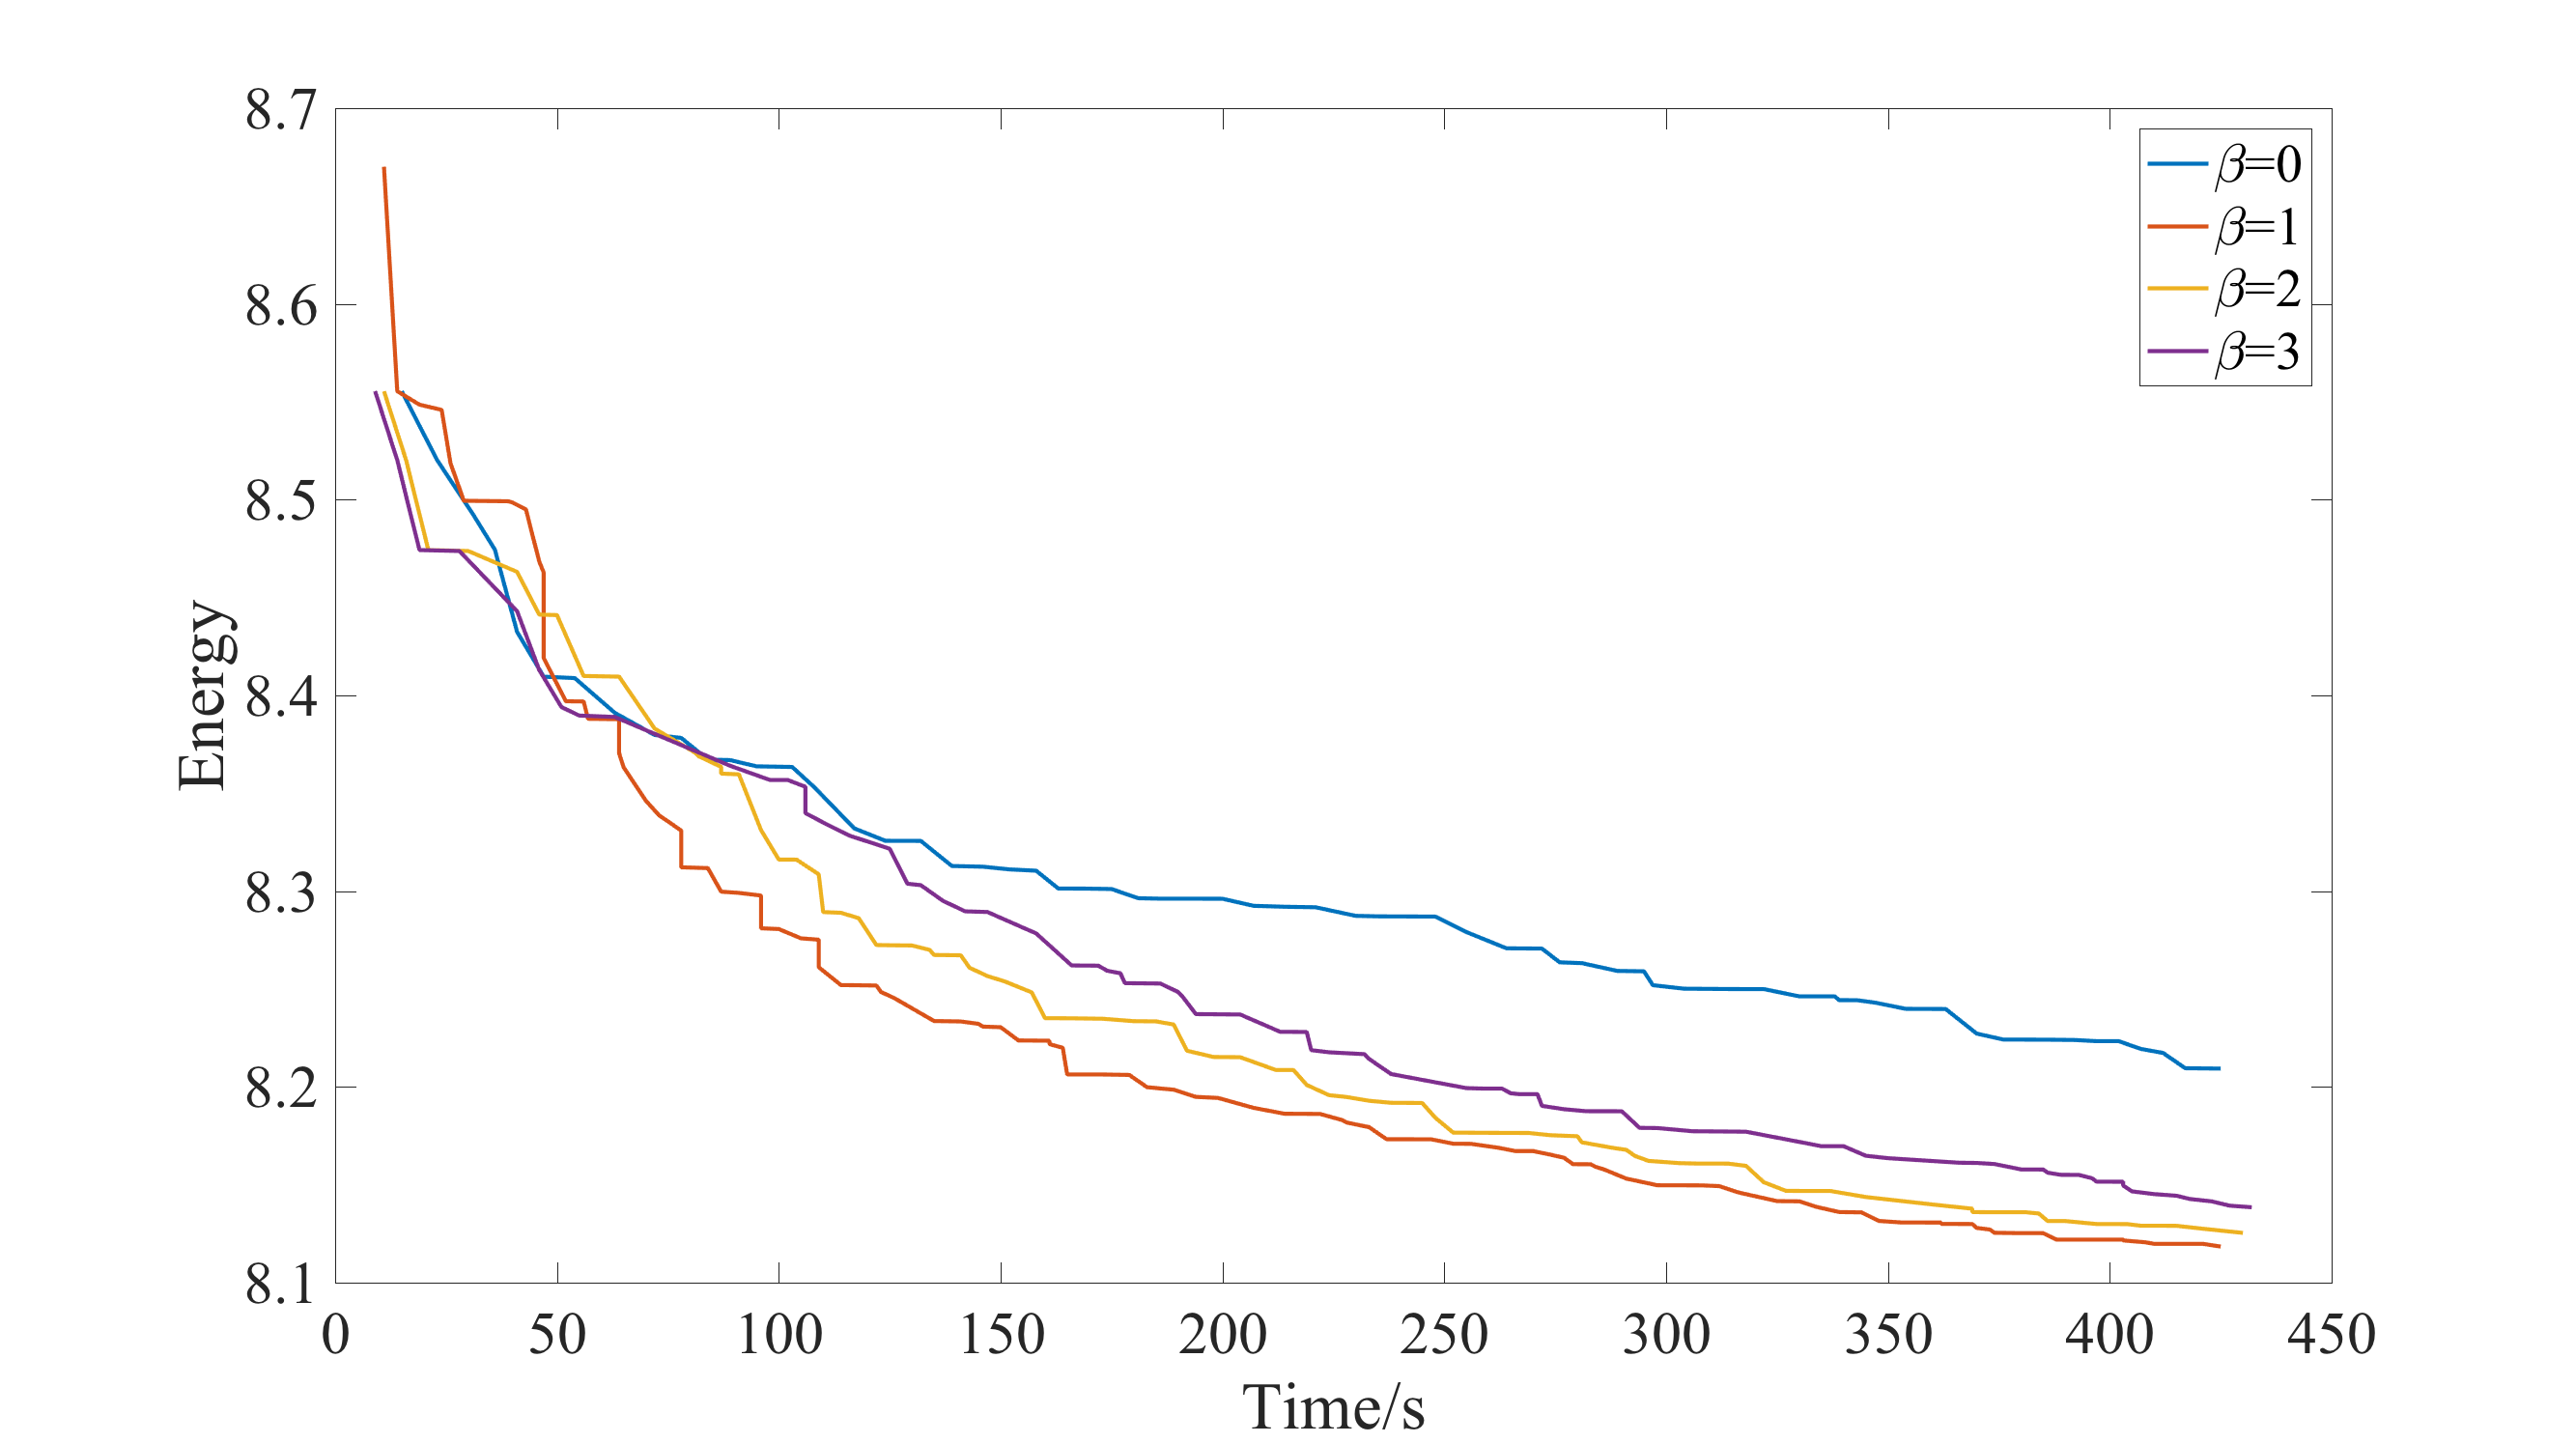
\includegraphics[width=\columnwidth]{figure/optical_flow_by_beta.png}
  \caption{}\label{fig:optical_flow_by_beta}
\end{figure}
\begin{figure}[tb]
  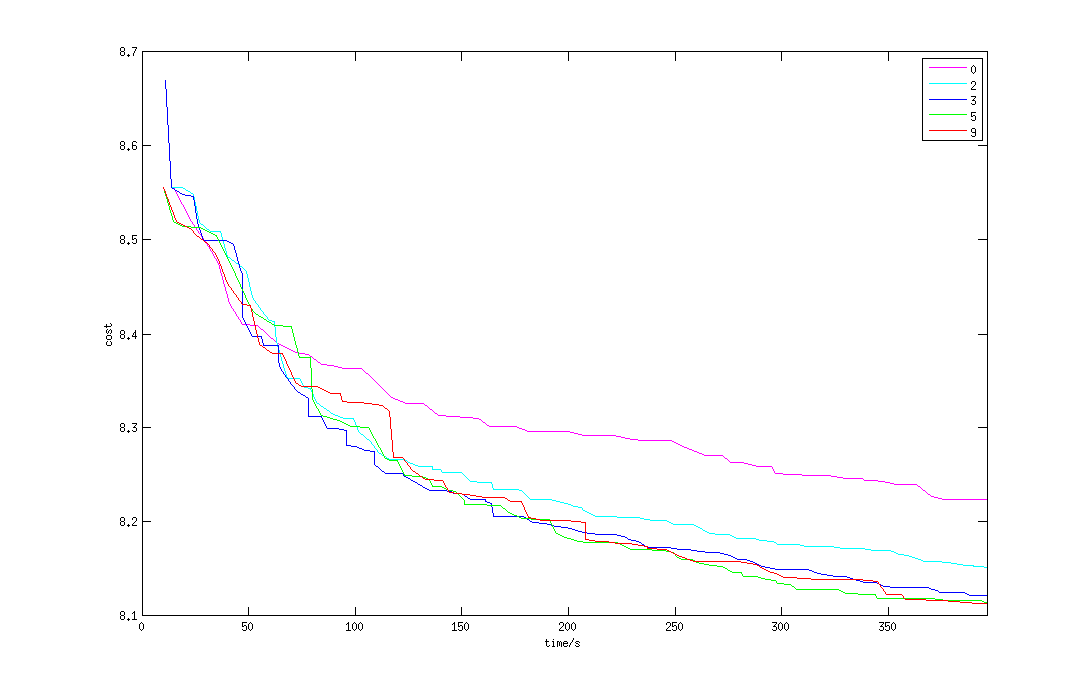
\includegraphics[width=\columnwidth]{figure/optical_flow_by_interval.png}
  \caption{}\label{fig:optical_flow_by_interval}
\end{figure}


\chen{
  There are interesting pattern in the convergence plot of optical flow estimation problem. As both FS-MF and PAE are doing binary fusion, FS-MF finds lower energy faster than PAE. The reason is as follows. Some solution proposals are more effective than others, so once a thread grabs an effective solution proposal, it find a much lower energy. Since there is no solution sharing in PAE model, other threads cannot share this lower energy state, and keeps working on improving its own state. On the other hand, FS-MF allows solution sharing, so once a thread grabs an effective solution proposal and moves to a lower energy state, other threads can share this lower energy state. To further demonstrate what is happening here, we plot the energy-time for each thread in PAE and FS-MF in figure \ref{fig:optical_flow_by_threads}. As we can see from the plots, in PAE model, one thread finds lower energy state faster than others, while other threads keep working at their own energy state. But in FS-MF model, all threads exchange information about the lowest energy state and work on improving the lowest energy state together. So there are more chance of finding effective proposals faster and thus the energy goes down faster. Since the solution for optical flow can be locally improved by each thread, the final merging of PAE can effectively fuse good local results in different threads together and achieve a similar energy state with FS-MF model. Because FS-MF model shares information in the middle, a final merging becomes less necessary. Same comparison holds for FS-SS and FS.
}

\chen{
  To further understand the effect of solution sharing, we did two other experiments. In one experiment, we change the number of solutions each thread grabed from others from 0 to 3 (as there are 4 threads in total) while keeping others the same. The energy-time plots are shown in figure \ref{fig:optical_flow_by_beta}. As shown in the figure, energy decreases faster with solution sharing. While since we need to perform one fusion for sharing each solution, sharing more solution leads to unnecessary overhead in this problem setting. While sharing multiple solutions might be benefitial in some problem setting as it means each thread can get more global information early. In another experiment, we change the number of iterations between two consecutive solution sharing iterations as in figure \ref{fig:optical_flow_by_interval}. From the figure, we can see that although solution sharing generally speed up the optimization process, sharing solution too frequently is not a good practice. This is because When we share solution frequently, we have less time for generating and fusing new proposals. A good choice of the solution sharing frequency depends on specific problem setting.
}

\chen{
  From the convergence plot of layered depth map estimation, we can see that, Fusion Move, Parallel Fusion Move, and FS-MF all stalk at a high energy state. The reason is binary fusion of solution proposals (either from others or self) is too limited to further decrease the energy due to the complexity of the problem itself. Only when multi-way fusion is used (in FS-SS and FS), it becomes possible for the energy to further decrease. This coincides with the observation in \cite{layered_depthmap} that binary fusion of proposal solutions is not as powerful as their subspace fusion which is a special form of multi-way fusion here. To further explore the effect of multi-way fusion, we use different $\alpha$ {1, 3, 7, 15} in FS model while keeping other parameters the same and plot the energy-time curve in figure \ref{fig:layered_depth_map_by_alpha}.
}

\chen{
  As shown in \ref{section:results}, the multi-way fusion and solution sharing enabled by our uniform framework play a key role for improving performance in different settings. For better understanding our framework, we examine the role played by each factor more closely by varying each factor while keeping others the same. There are four parameters in our framework: \textit{the number of threads}, \textit{the number alpha}, \textit{the number beta}, \textit{the number of iterations between each solution sharing}.
}


\section{Conclusion and future directions}
We have proposed a novel MRF inference framework, Swarm Fusion, in
parallel computing environments. The framework is general and makes
popular inference techniques such as Alpha Expansion, Fusion Move,
Parallel Alpha Expansion, and Hierarchical Fusion, its special cases. Our
experiments have revealed that the framework exploits parallel
computational resources and achieves faster convergence, especially for
challenging problems.  Our first future work is to conduct experiments
on cloud computing environments, in particular, the MapReduce
programming model, where the roles of mappers and reducers exactly
correspond to the processes of parallel multi-way fusion and solution
sharing, respectively.  Another future work is the automatic
configuration of the Swarm Fusion architecture.  Our experiments have
shown that optimal architectures are different for different problems.
An interesting direction is to adaptively change its architecture during
the computation, for example, switching to simple parallel
alpha-expansion for easy problems, or increasing the rate of solution
exchanges when solutions vary significantly across threads.
%
Parallel MRF inference has been a relatively under-explored topic in
Computer Vision.
%
%Our idea is very simple, where adapting the Swarm Fusion
%framework require minimal coding.
%
The proposed Swarm Fusion framework can be intergrated into existing
algorithms with minimal coding.  We believe that this paper would
immediately benefit tens of thousands of Computer Vision researchers
or engineers in the world, who currently solve MRF problems. We will
share our source code with the community.


\bibliographystyle{splncs}
\bibliography{eccv16bib}
\end{document}
